\documentclass[12pt]{article}
\usepackage[english]{babel}
\usepackage[utf8]{inputenc} % Permite el uso de caracteres del Español
\usepackage[T1]{fontenc}
\usepackage{graphicx}
\usepackage{amsmath}
\usepackage{wrapfig}
\usepackage{enumerate}
\usepackage[top=1in, bottom=1.25in, left=1.1in, right=1.1in]{geometry}
\usepackage[dvipsnames]{xcolor}
\usepackage{subcaption}

\begin{document}

\begin{titlepage}

\newcommand{\HRule}{\rule{\linewidth}{0.5mm}} % Define un comando para las lineas horizontales

\center 
%----------------------------------------------------------------------------------------
%	Cabezera
%----------------------------------------------------------------------------------------

\textsc{\LARGE Universidad de Sonora}\\[1.5cm]
\textsc{\Large Licenciatura en Física}\\[0.5cm]
\textsc{\large Física Computacional I}\\[0.5cm]

%----------------------------------------------------------------------------------------
%	Titulo
%----------------------------------------------------------------------------------------

\HRule \\[0.4cm]
{\huge \bfseries Actividad 4 - Introducción a la programación de los intérpretes de comandos.}\\[0.4cm] % Title of your document
\HRule \\[1.5cm]
 
%----------------------------------------------------------------------------------------
%	Autor
%----------------------------------------------------------------------------------------

\begin{minipage}{0.4\textwidth}
\begin{flushleft} \large
\emph{Alumno:}\\
José Gabriel Navarro I.
\end{flushleft}
\end{minipage}
~
\begin{minipage}{0.4\textwidth}
\begin{flushright} \large
\emph{Profesor:} \\
Carlos Lizarraga Celaya
\end{flushright}
\end{minipage}\\[2cm]


%----------------------------------------------------------------------------------------
%	Fecha
%----------------------------------------------------------------------------------------
21 de Febrero de 2018

%----------------------------------------------------------------------------------------
%	Escudo
%----------------------------------------------------------------------------------------


\includegraphics[width=0.4\textwidth]{logo.png}\\
 
%----------------------------------------------------------------------------------------

\vfill % Llena el espacio de la pagina en blanco

\end{titlepage}

\section{Introducción}
En el presente reporte se habla acerca de la cuarta actividad realizada para la clase de Física Computacional I, el cual abarca el uso de un interprete de comandos de UNIX llamado Shell. En la actividad se realizaron distintas acciones con este interprete como es la descarga de datos, su organización y filtración, además de la creación de archivos.\\ 

En el reporte se habla acerca del proceso realizado en la practica ademas de su resultado al utilizar varios comandos en el interprete, como lo fue el uso de  cat, chmod, echo, grep entre otros. También se da una pequeña descripción de cada uno de ellos de manera teórica. Además de esto se presenta una síntesis acerca de un tutorial de Shell, en donde se muestran varios ejemplos presentados en la pagina web. 

\section{Actividades realizadas}
Primeramente se descargo el archivo proporcionado por el profesor. Este archivo es un script que permite descargar todos los registros de los días en un año de una estacion seleccionada de los sondeos climáticos. El script fue editado de manera que la estación seleccionada fuera la misma estación que la practica anterior: Observatorio de Valentia. \\ \\

El script se muestra a continuación:

\begin{center}
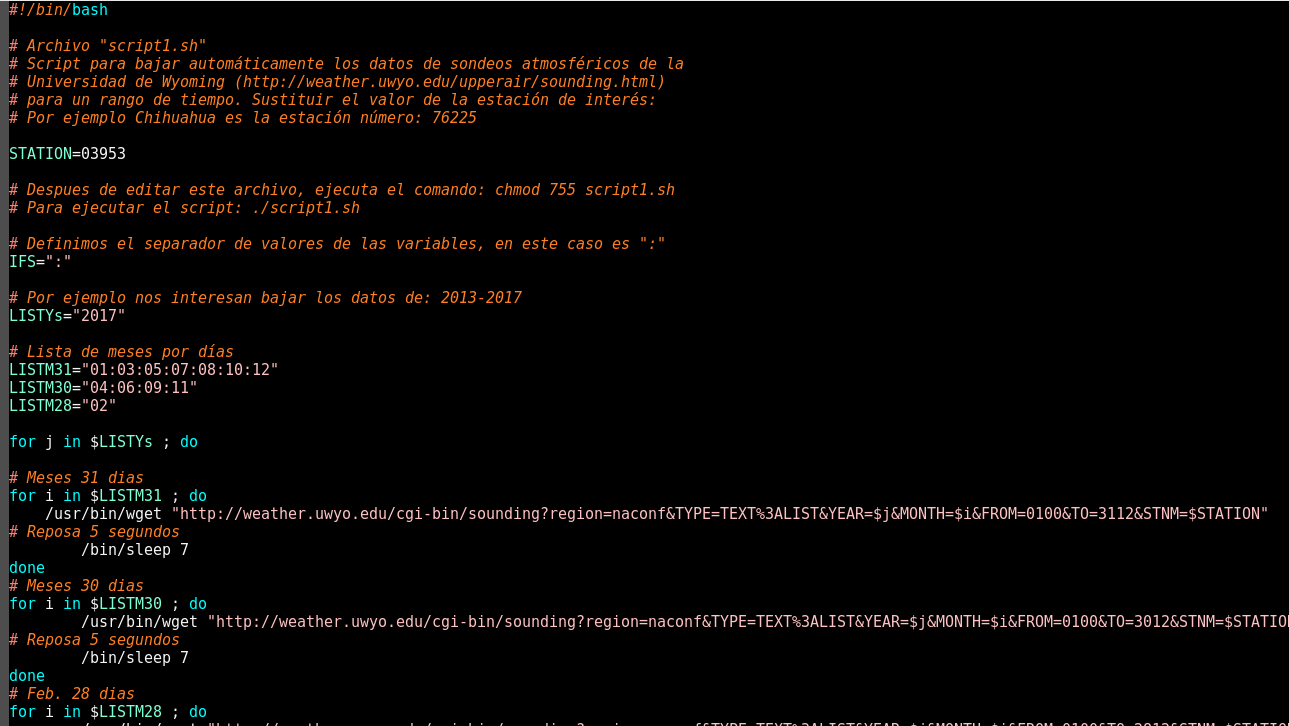
\includegraphics[scale=0.5]{Script.png}
\end{center} 

La función de este script, como ya se había mencionado, es descargar todos los registros del año del sondeo meteorológico de una estación, el Observatorio de Valentia en mi caso. Podemos observar como en el script, primero se declaro como variable a la estación y los distintos meses dependiendo del numero de días que tiene, esto para que al descargar los datos no se descargue datos basura. Posteriormente en los ciclos 'DO', podemos observar como dependiendo del mes que es es el numero de veces que se repite el proceso, cambiando el URL de descarga dependiendo de la estación y del mes. Para descargar los datos se utiliza el comando wget. \\ 

Sin embargo, el script aun no es un ejecutable, utilizando el comando \textit{\textbf{ls- alg}} nos muestra los permisos del archivo, en donde podemos observar que solo es para lectura y edición. Los permisos del archivo se clasifican de la siguiente manera:

\begin{center}
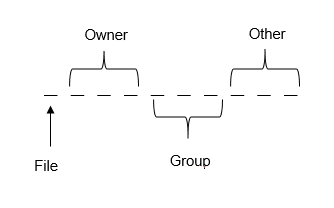
\includegraphics[scale=0.7]{Tipo_de_archivo.png}
\end{center} 

Al realizar este comando, observamos que el archivo tiene los permisos:  -rw-r--r--, que significa que es solamente de lectura para el dueño. Para cambiarlo a ejecutable se utiliza  el comando  \textit{chmod} que permite cambiar los permisos de un archivo, usando la notación numérica en base 8. Entonces, para cambiarlo a un ejecutable usamos la notación 755, en donde el resultado será:

\begin{center}
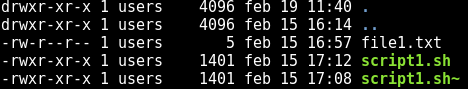
\includegraphics[scale=0.7]{ejecutable.png}
\end{center} 

Ahora que es un ejecutable, al correrlo se empieza a descargar todos los archivos, un total de 12 archivos, mostrando el progreso de descarga en cada uno y tomándose un descanso cada 7 segundos entre archivos. El resultado obtenido fue:

\begin{center}
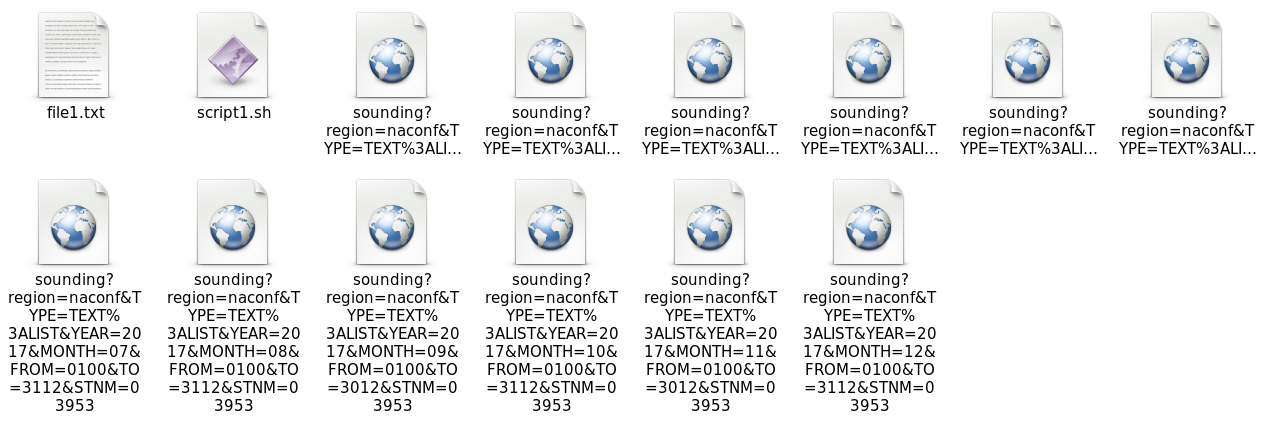
\includegraphics[scale=0.45]{Archivos.png}
\end{center} 

\begin{center}
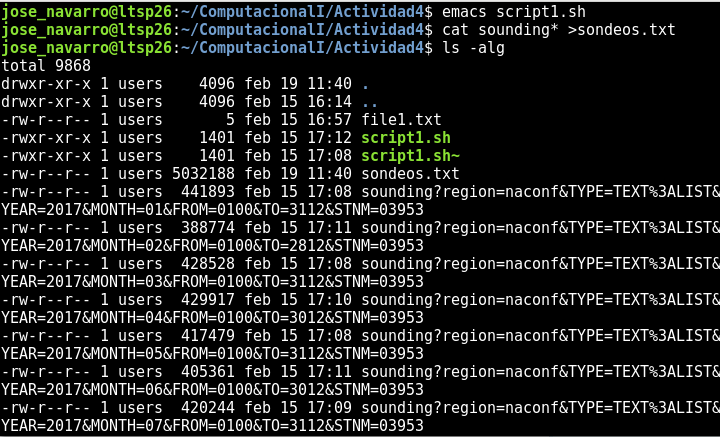
\includegraphics[scale=0.55]{ls_-alg.png}
\end{center} 

Para la lectura y revisión, se utilizaron dos comandos, uno de ellos es  \textbf{\textit{less}}. Este comando muestra en la terminal todos los datos de un solo archivo en pantalla, pero muestra todo seguido, es decir, la terminal no baja hasta el punto final, permite examinar todos los datos de inicio a fin, pero solamente permite la visualización de la información, no permite editarlos. Por otro lado el comando  \textbf{\textit{cat}} muestra todos los datos en pantalla, al igual que less, pero este pone el cursor al final del archivo, de manera que permite visualizar desde del fin del archivo hacia arriba en si concatena los datos para mostrar la información del archivo. \\

\begin{center}
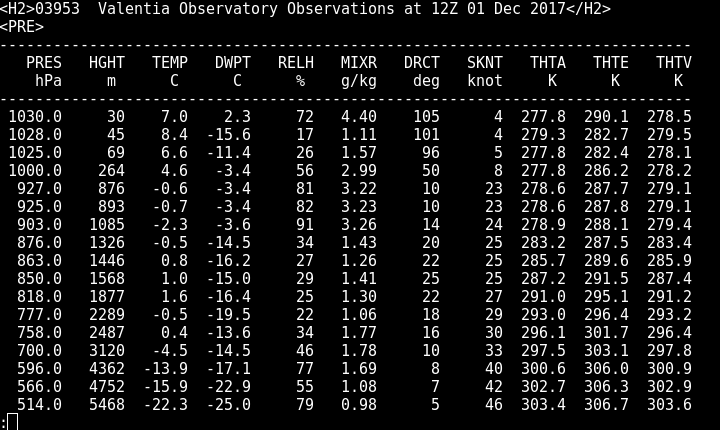
\includegraphics[scale=0.55]{less.png}
\end{center} 

El comando  \textbf{\textit{grep}} permite tomar información en especifico de un archivo por renglón. Esto se hace indicando el comando, la palabra a buscar y el archivo de donde se obtendrá esa información. Esto puede hacerse con varias palabras, de distintos archivos e incluso limitarlo aun cierto numero de renglones. grep significa global regular expression print, ya que se usa en su mayoría para buscar texto o buscar en archivos lineas especificas. \\

\begin{center}
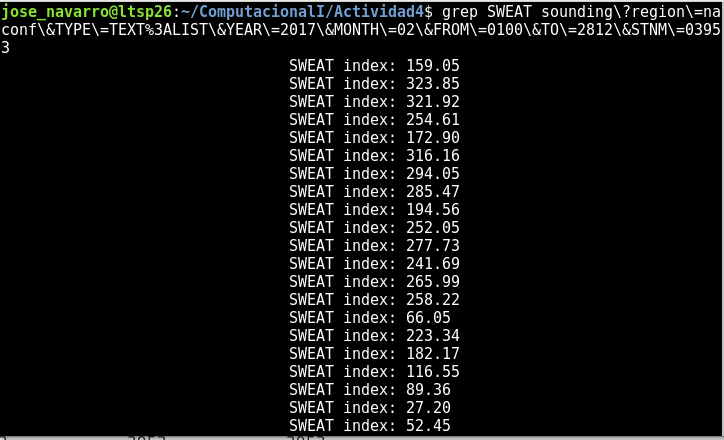
\includegraphics[scale=0.55]{grep.png}
\end{center} 

Ahora vamos a juntar todos estos archivos en uno solo. Utilizando el comando  \textit{ file sounding*}, podremos ver el tipo de archivo que hay en nuestra carpeta enfocándose solamente en los archivos que comiencen con sounding, en este caso es un archivo de texto ASCII:

\begin{center}
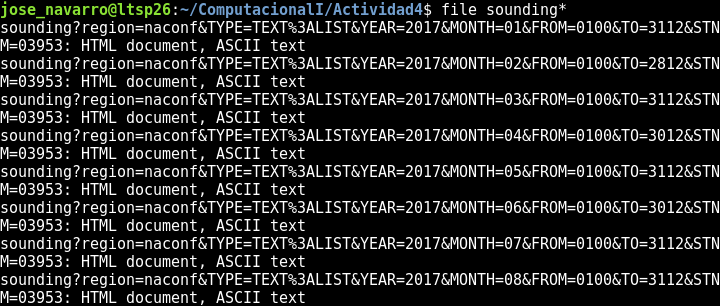
\includegraphics[scale=0.55]{ascii.png}
\end{center} 

Para juntar todos los archivos en uno solo usaremos el comando cat de nuevo pero esta vez usaremos el redirector > para indicar que todos estos archivos irán a un archivo .txt. De esta manera queda creado el archivo. \\

Ahora para obtener solamente los renglones que deseamos, utilizaremos el comando grep, seleccionando solamente los renglones que estan al final de la tabla. Como ya se había mencionado, grep permite elegir renglones con distintas palabras, esto mediante el uso de |, separando las palabras a buscar. El comando en si es:

\begin{verbatim}
egrep -v 'PRES|hPa' sondeos.txt | egrep '76225|Showalter...Precip' > df2017.csv \\
\end{verbatim}

En donde el indicador -v significa que va tomar todos los datos excepto los que contengan las palabras PRES y hPa. Mientras que el resto del código toma los renglones que presenten las palabras Sowalter, Precip, etc.\\

Estas ultimas dos acciones realizadas pueden ser automatizadas mediante el uso de un script. Si creamos un script que contenga estas dos indicaciones, y cambiándolo a un ejecutable, estas acciones podrán hacerse rápidamente sin la necesidad de hacerlo manualmente. Para esto solo se creo un archivo de emacs con terminación sh, se puso los comandos anteriormente mencionados, con un cambio solamente en el archivo de destino, ahora siendo df2017\_2.csv. Posteriormente se convirtió a un ejecutable y se corrió. Esto genero el archivo que se muestra a continuación. 

\begin{center}
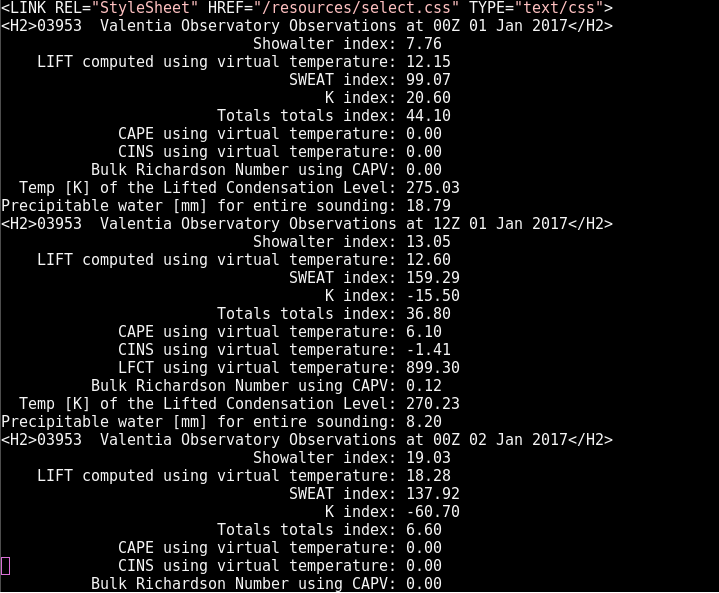
\includegraphics[scale=0.55]{archnuevo.png}
\end{center} 

Este archivo deberia ser exactamente igual al creado anteriormente mediante el método manual, para comprobar esto se uso el comando \textbf{\textit{diff}}, el cual indica la diferencia entre dos archivos. Si existe una diferencia se mostrara en pantalla, si no lo hay, no se muestra nada como se observa a continuación: \\

\begin{center}
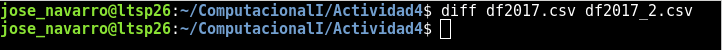
\includegraphics[scale=0.55]{diff.png}
\end{center} 

Algunos comandos utilizados también fueron los de ls, wc y echo. \textbf{\textit{echo}}permite escribir o mandar información aun archivo, por ejemplo, se puede crear un archivo y dentro de el se puede escribir algo utilizando este comando, además también permite visualizar la ubicación en donde se encuentra actualmente la terminal:

\begin{center}
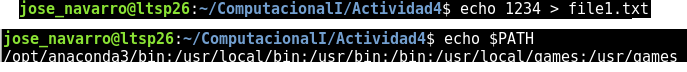
\includegraphics[scale=0.55]{echo.png}
\end{center} 

\textbf{\textit{Ls}} se utilizo mucho al revisar los archivos y sus permisos, esto es porque ls permite ver el contenido de los directorios, y agregando -alg, permite vernos también los permisos que tiene. \\

\textbf{\textit{wc}} imprime en pantalla el numero de lineas, palabras o bytes en un archivo, esto indicado ya sea por c, l o w, seguido por el nombre del archivo, por ejemplo, en este archivo hay 5632 lineas:

\begin{center}
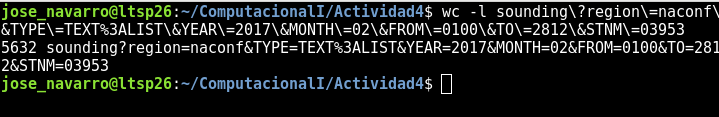
\includegraphics[scale=0.55]{wc.png}
\end{center} 

\section{Síntesis}
A continuación se presenta la síntesis de la pagina Shell Script, donde se muestra un poco de teoría acerca del tema y posteriormente algunos ejemplos:

\subsection{Introducción y Filosofía}
La programación de Shell tiene un poco de mala fama entre algunos sistemas administrativos de Unix. Esto se debe a la rapidez en la que un programa interpretado corre a comparación de un programa en C, en C es mas rápido y por tanto preferible, y como es muy fácil escribir este tipo de scripts, existen muchos scripts de shell de poca calidad. \\

Es por eso que es importante que el script a realizar sea claro y legible, tratando de evitar comandos innecesarios. Esto ya que el sistema operativo tarda mas, entre mas comandos tenga que realizar.  

\subsection{Un primer script}
Para el primer script a realizar, haremos el programa clásico: "Hola Mundo". Para esto solamente crearemos un script con lo siguiente:

\begin{verbatim}
#!/bin/sh
# Este es un comentario!
echo Hola Mundo        # Los comentarios en casi cualquier lugar!
\end{verbatim}

La primera linea le dice a Unix que el archivo debe ser ejecutado en 
\textbackslash bin\textbackslash sh, La segunda linea indicada por un \#, es un comentario, y es ignorada por Shell, siendo la única excepción cuando este símbolo esta acompañado por !, lo cual significa que no importa que shell estemos utilizando este debe de ser interpretado por el Shell original. Por ultimo el tercer renglón contiene el comando echo, el cual imprime en pantalla lo que se escribe después del punto. \\

\begin{center}
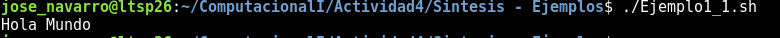
\includegraphics[scale=0.55]{Ej1_1.png}
\end{center} 

Algo a notar, es que echo automáticamente puso un espacio entre las palabras, pero si colocamos mas espacios shell lo interpretara como solamente uno, para poder realizar cambios de este estilo, debemos de colocar el texto entre comillas:

\begin{verbatim}
#!/bin/sh
# Este script muestra las diferencias al usar las comillas en el comando echo
echo "Hola 		Mundo"
echo Hola mundo
\end{verbatim}

Aquí se puede notar la diferencia: 

\begin{center}
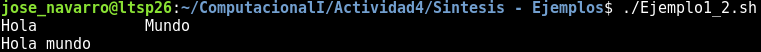
\includegraphics[scale=0.55]{Ej1_2.png}
\end{center} 

\subsection{Variables}
En casi todos los lenguajes de programación existe el concepto de variables, un nombre simbólico a un trozo de memoria al cual podemos asignarle un valor, leer y manipular su contenido. Para asignar variables se debe de igualar el nombre de la variable a lo que se desea almacenar, pero sin espacios. \\

A shell no le importa el tipo de variable, pueden contener caracteres, enteros, reales, lo que se necesite. Pero si sabe diferenciar entre ellos; no se puede hacer la suma de un carácter y un numero. Inclusive se puede utilizar variables junto con el comando read para interactuar con la computadora:

\begin{verbatim}
#!/bin/sh
echo ¿Cuál es tu nombre?
read NOMBRE
echo "Hola $NOMBRE - espero estes bien!"
\end{verbatim}

\begin{center}
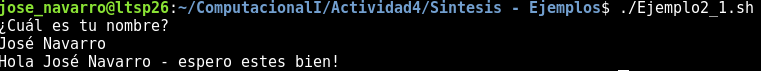
\includegraphics[scale=0.55]{Ej2_1.png}
\end{center} 

Si se declaran mal las variables el script no marcara error, si no que se imprimirá en pantalla la cadena de carácter vació, es decir, nada. Si se quiere utilizar variables declaradas DESPUÉS de su impresión, es necesario exportarlas, ya que cada vez que corremos nuestro script, el shell se reinicia y pierde el valor.  \\

Ahora bien, no se puede usar el nombre o contenido de una variable uniéndola a otra, es decir, no podemos nombrar algo con nuestra variable a menos que se utilicen corchetes como se indica:

\begin{verbatim}
#!/bin/sh
echo "¿Cuál es tu nombre?"
read USUARIO
echo "Que onda $USUARIO"
echo "Creare una archivo con el nombre ${USUARIO}_archivo"
touch "${USUARIO}_archivo"
\end{verbatim}

\begin{figure}[h!]
\begin{subfigure}{.55\textwidth}
  \centering
  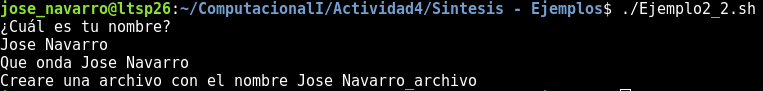
\includegraphics[width=.8\linewidth]{Ej2_21.png}
  \caption{Impresión en pantalla}
  \label{fig:sfig1}
\end{subfigure}
\begin{subfigure}{.55\textwidth}
  \centering
  
\includegraphics[width=.55\linewidth]{Ej2_22.png}
  \caption{Archivo creado}
  \label{fig:sfig2}
\end{subfigure}
\end{figure}

\subsection{Wildcards (Comodines)}
Estos son solamente comandos para utilizar en la terminal para facilitar el movimiento y edición de archivos de distintas sintaxis. Por ejemplo, si queremos copiar todos los archivos de una carpeta 'a'  otra carpeta 'b' podemos utilizar:

\begin{verbatim}
cp /tmp/a/* /tmp/b/
cp /tmp/a/*.txt /tmp/b/
cp /tmp/a/*.html /tmp/b/
\end{verbatim}

\begin{figure}[h!]
\begin{subfigure}{.55\textwidth}
  \centering
  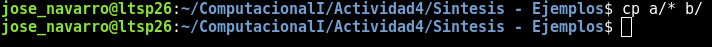
\includegraphics[width=.8\linewidth]{Ej3_11.png}
  \caption{Impresión en pantalla}
  \label{fig:sfig1}
\end{subfigure}
\begin{subfigure}{.55\textwidth}
  \centering
  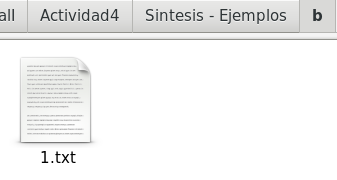
\includegraphics[width=.8\linewidth]{Ej3_12.png}
  \caption{Archivo de carpeta A a B}
  \label{fig:sfig2}
\end{subfigure}
\end{figure}

O si queremos imprimir en pantalla la lista de archivos en una carpeta, pero sin utilizar ls, podemos usar un echo \textbackslash tmp\textbackslash a\textbackslash *. \\

Generalmente se utilizan las "wildcards" para facilitar el movimiento de archivos, y casi no se usan en scripts.

\subsection{Caracteres de Escape}
Algunos caracteres tienen significado en shell, por ejemplo, las dobles comillas afectan en como se tratan los espacios en el comando echo. Pero si deseamos utilizar las comillas como texto, ¿cómo lo hacemos?

\begin{verbatim}
$ echo "Hello   \"World\""
\end{verbatim}

Esto permite imprimir: Hello    "World", que era lo deseado.  \\

\begin{center}
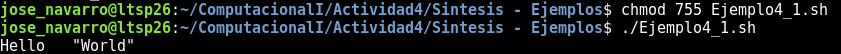
\includegraphics[scale=0.55]{Ej4_1.png}
\end{center} 

La mayoría de los caracteres no son interpretados como texto, para eso tienen que ser colocados entre comillas, si no el interpretador los toma como código.

\begin{verbatim}
echo * 
echo *txt
echo "*" 
echo "*txt"
\end{verbatim}

En el primer renglón, * imprimirá todos los archivos en el directorio, y *txt imprimirá todos los archivos .txt en pantalla. Mientras que en el renglón 3 y 4 se imprimirá el carácter. Sin embargo, algunos caracteres como \$ y ' aun son interpretados por shell. Es por eso que se utiliza el carácter \textbackslash para su uso, tal como se muestra en el primer ejemplo. 

\begin{center}
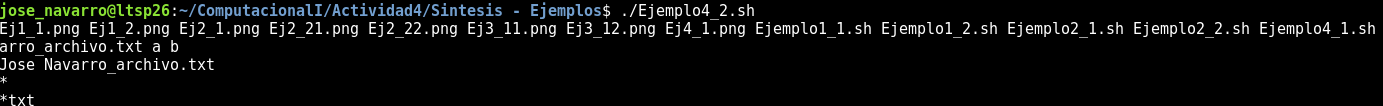
\includegraphics[scale=0.35]{Ej4_2.png}
\end{center} 

\subsection{Ciclos}
La mayoría de los lenguajes tienen lo que son los ciclos. Si queremos repetir algo veinte veces, no tenemos que escribir el código 20 veces cambiándolo un poco cada vez. Existen dos tipos de ciclos, los "for" y los "while"

\subsubsection{Ciclos For}
Estos ciclos iteran hasta que la lista de valores se acabe, los valores pueden ser cualquier cosa, por ejemplo, el siguiente código imprime en pantalla con un carácter, numero, después toma todos los archivos del directorio actual, numero y por ultimo carácter:

\begin{verbatim}
#!/bin/sh
for i in Hola 1 * 2 bye-bye 
do
  echo "Ciclando... i tiene el valor $i"
done
\end{verbatim}

\begin{center}
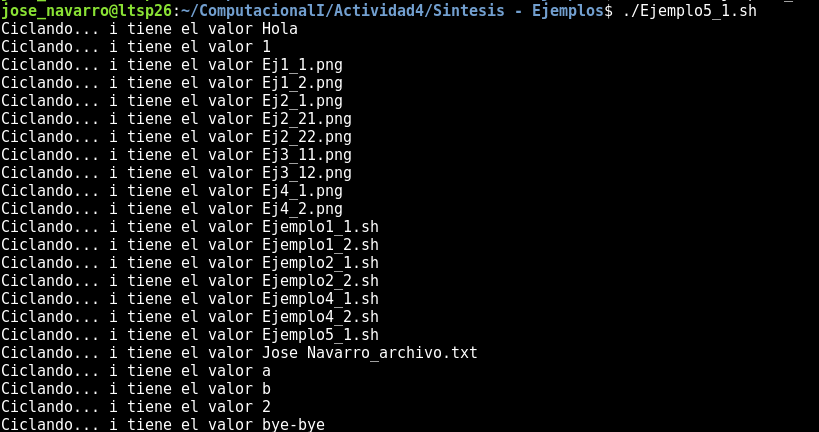
\includegraphics[scale=0.5]{Ej5_1.png}
\end{center} 

\subsubsection{Ciclos While}
En estos ciclos, las instrucciones dentro de este se repetirán indefinidamente hasta que se cumpla la condición de salida, por ejemplo, el siguiente código muestra un ciclo que seguirá hasta que el usuario escriba "bye", si no, el ciclo sigue indefinidamente: 

\begin{verbatim}
#!/bin/sh
CARACTER=hola
while [ "$CARACTER" != "bye" ]
do
  echo "Escribe algo (escribe bye para salir)"
  read LETRAS
  echo "You typed: $LETRAS"
done
\end{verbatim}

\begin{center}
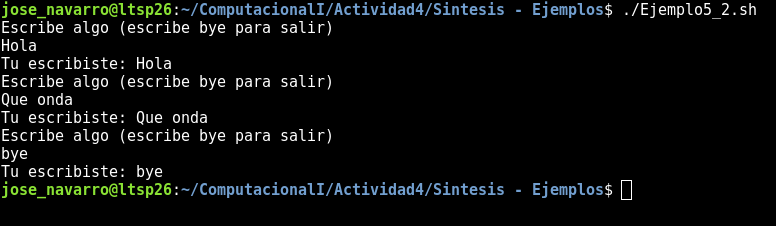
\includegraphics[scale=0.5]{Ej5_2.png}
\end{center} 

\section{Bibliografía}
\begin{itemize}
    \item Ls command in Linux.(2018) Recuperado de: www.rapidtables.com/code/linux/ls.html
    \item Wc. (2014) Recuperado de: www.tutorialspoint.com/unix\_commands/wc.htm
    \item Shell Scripting Tutorial. (2018). Recuperado de: www.shellscript.sh/index.html
\end{itemize}

\section{Apéndice}
\noindent\textbf {1. ¿Qué fue lo que más te llamó la atención en esta actividad?} \\ \\
Utilizar nuevos comandos en el interprete de comandos de UNIX. Anteriormente en Fortran las primeras practicas consistieron en el uso de estos comandos para creación de carpetas y archivos, pero esto comandos son mucho mas avanzados. Esto sin mencionar el uso de los scripts una herramienta muy util para automatizar estos mismo comandos. \\

\noindent\textbf {2. ¿Qué consideras que aprendiste?}\\ \\
El uso de scripts para automatizar procesos y aprender a hacer manualmente estos procesos. \\ 

\noindent\textbf {3. ¿Cuáles fueron las cosas que más se te dificultaron? } \\ \\
Entender la sintaxis de los comandos, cada uno es distinto y tiene  su forma de trabajar, lo cual dificulta un poco en aprenderse que hace cada uno y su forma de usarlo. \\

\noindent\textbf {4. ¿Cómo se podría mejorar en esta actividad?} \\ \\
Una pequeña introducción teórica al uso de los comandos y de donde se originan, para así tener contexto de su uso y abreviaciones. \\ \\

\noindent\textbf {5. ¿En general, cómo te sentiste al realizar en esta actividad? }\\  \\
Me sentí bien, un poco inseguro debido a que es algo que no había visto antes y me daba miedo no saber manejarlo, pero con la investigación y bibliografía, ademas de la ayuda del profesor y compañeros salio todo bien.
\end{document}